\documentclass[aspectratio=169, table]{beamer}

\usepackage[utf8]{inputenc}
\usepackage{listings} 

\usetheme{Pradita}

\subtitle{MTI104 - IT Services}

\title{Session-01:\\\LARGE{Practices to Manage Changes\\}}
\date[Serial]{\scriptsize {PRU/SPMI/FR-BM-18/0222}}
\author[Pradita]{\small{\textbf{Alfa Yohannis}}}

\begin{document}

\frame{\titlepage}

\begin{frame}
	\frametitle{Importance of Change}
	\begin{itemize}
		\item Operations maintain the status quo.
		\item Services or products need to evolve.
		\item Without changes, services/products become obsolete.
		\item Even simple products like confectionaries evolve.
		\item Example: Avatars of Haribo or chocolates change frequently.
		\item Exception: "Classic" Coke returned due to popular demand.
		\item IT products/services need constant improvement to survive.
	\end{itemize}
\end{frame}

\begin{frame}
	\frametitle{Managing Change in IT}
	\begin{itemize}
		\item Introducing changes requires careful planning.
		\item Principles, processes, practices, and procedures are essential.
		\item Users accustomed to a certain way of doing things may resist change.
		\item Change must minimize disruption to services.
		\item ITIL provides a framework for managing changes safely.
		\item Desire to change is high; appetite for risk is low.
		\item This chapter covers practices to manage change.
	\end{itemize}
\end{frame}

\begin{frame}
	\frametitle{ITIL Practices Covered}
	\begin{itemize}
		\item Two key practices discussed:
		\item Service request management
		\item Change control
		\item Understanding these practices is crucial for IT careers.
		\item Change control is as important as incident management.
		\item ITIL Foundation exam heavily focuses on these topics.
		\item Expect 7-8 questions from this chapter in the exam.
	\end{itemize}
\end{frame}

\begin{frame}
	\frametitle{Service Request Management}
	\begin{itemize}
		\item Minor practice often confused with incident management.
		\item ITIL defines service request management.
		\item Purpose: Support agreed service quality.
		\item Handles predefined, user-initiated service requests.
		\item Ensures service requests are fulfilled based on agreed levels.
		\item Service requests must be well-defined.
		\item Understanding service requests is crucial.
	\end{itemize}
\end{frame}

\begin{frame}
	\frametitle{Examples of Service Requests}
	\begin{itemize}
		\item Requesting a new checkbook from a bank.
		\item Installing open-source software on a laptop.
		\item Requesting access to a portal.
		\item Asking for information, e.g., directions to a location.
		\item Providing compliments, complaints, or feedback.
		\item Service request is not a complaint or incident.
		\item Service request management was known as request fulfillment in ITIL V3.
	\end{itemize}
\end{frame}

\begin{frame}
	\frametitle{Service Catalog and Incident Confusion}
	\begin{itemize}
		\item Service requests must be predefined.
		\item Users can't request undefined services.
		\item All service requests are listed in the service catalog.
		\item Service catalog must be shared with users.
		\item Incidents and service requests were once treated the same.
		\item Incident: Loss of service; Service request: Getting something additional.
		\item Treating them the same increases service downtime.
	\end{itemize}
\end{frame}

\begin{frame}
	\frametitle{Fulfillment of Service Requests}
	\begin{itemize}
		\item Service requests are predefined and straightforward.
		\item Standard operating procedures (SOPs) are used for fulfillment.
		\item Example service requests: Laptop request, software installation, experience letter.
		\item Each request follows a different flow and involves different teams.
		\item Portal used for initiating service requests.
		\item Automation can enhance the efficiency of request fulfillment.
		\item Service requests are a form of standard changes.
	\end{itemize}
\end{frame}

\begin{frame}{Fulfilment of service requests}
	 \frametitle{Fulfilment of service requests}
\begin{center}
	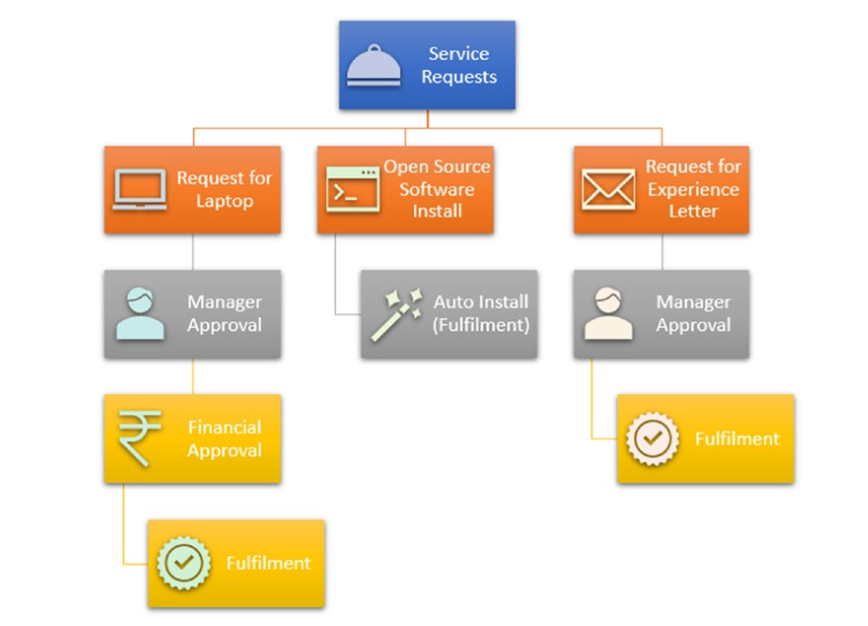
\includegraphics[width=0.5\linewidth]{images/image-01.png}
\end{center}
\end{frame}

\begin{frame}
	\frametitle{Guidelines for Service Request Management}
	\begin{itemize}
		\item Clear boundaries for service requests, incidents, and changes.
		\item All service requests must be clearly defined.
		\item Service catalog should be available to all users.
		\item Standardize service request flows where possible.
		\item Automate service requests that don't need human intervention.
		\item Service request management should be continuously improved.
		\item Engage with the Service Value Chain (SVC) for better service.
	\end{itemize}
\end{frame}

\begin{frame}
	\frametitle{Change Control Practice}
	\begin{itemize}
		\item Change is constant and necessary in IT.
		\item Changes must be managed to avoid negative impacts.
		\item Mismanagement of changes can cause incidents.
		\item ITIL defines change as affecting service components.
		\item Components include servers, software, networks, etc.
		\item Managing changes requires careful consideration.
		\item Change control ensures changes are handled properly.
	\end{itemize}
\end{frame}

\begin{frame}
	\frametitle{Examples of Changes}
	\begin{itemize}
		\item Implementation of fiber optic Internet service
		\item Transition of email services from Exchange to Gmail
		\item Decommissioning of mainframe computers
		\item Adding extra memory to servers
		\item Changing ownership of a core switch
		\item Adding an IP to a blacklist on firewall
		\item Modification of a batch job
	\end{itemize}
\end{frame}

\begin{frame}
	\frametitle{Examples of Changes (cont.)}
	\begin{itemize}
		\item New version release of an iPhone app
		\item Upgrade of an enterprise application
		\item Changes in processes, governance, and IT staff
		\item Indirect effects on services
		\item Separate management of such changes
	\end{itemize}
\end{frame}

\begin{frame}
	\frametitle{ITIL Definition of Change Control Practice}
	\begin{itemize}
		\item Maximize successful service and product changes
		\item Ensure risks are assessed
		\item Authorize changes to proceed
		\item Manage the change schedule
		\item Govern changes to products and services
		\item Mitigate risks and increase change success
		\item Necessary for organizational improvement
	\end{itemize}
\end{frame}

\begin{frame}
	\frametitle{Change Control Example: Canary Testing}
	\begin{itemize}
		\item Release new app version to limited users
		\item Detect issues before full release
		\item Mitigate risks through controlled testing
		\item Ensure stability before wide deployment
	\end{itemize}
\end{frame}

\begin{frame}
	\frametitle{Scope of Change Control}
	\begin{itemize}
		\item ITIL does not specify scope boundaries
		\item Scope depends on service provider and customer
		\item Multiple elements managed by IT professionals
		\item Financial considerations impact scope
		\item Standard changes and service requests for peripheral objects
	\end{itemize}
\end{frame}

\begin{frame}
	\frametitle{Scope of Change Control (cont.)}
	\begin{itemize}
		\item Holistic approach to defining changes
		\item Categorization based on design aspects
		\item New or modified services
		\item Management information systems
		\item Technology and management architecture
		\item Policies, processes, and templates
		\item Measurement systems and KPIs
	\end{itemize}
\end{frame}

\begin{frame}
	\frametitle{Types of Changes}
	\begin{itemize}
		\item Different protocols for different changes
		\item ITIL categorizes changes into:
		\begin{itemize}
			\item Normal changes
			\item Emergency changes
			\item Standard changes
		\end{itemize}
		\item Custom types can be defined by organizations
	\end{itemize}
\end{frame}

\begin{frame}
	\frametitle{Normal Changes}
	\begin{itemize}
		\item Planned in advance
		\item Lengthy due to planning and stakeholder visibility
		\item Well analyzed, tested, mitigated, and verified
		\item Prioritization based on risk
		\item Example: Application refresh to a newer version
		\item Registered as a change request in ITSM tools
	\end{itemize}
\end{frame}

\begin{frame}{Change model}
	 \frametitle{Change model}
\begin{center}
	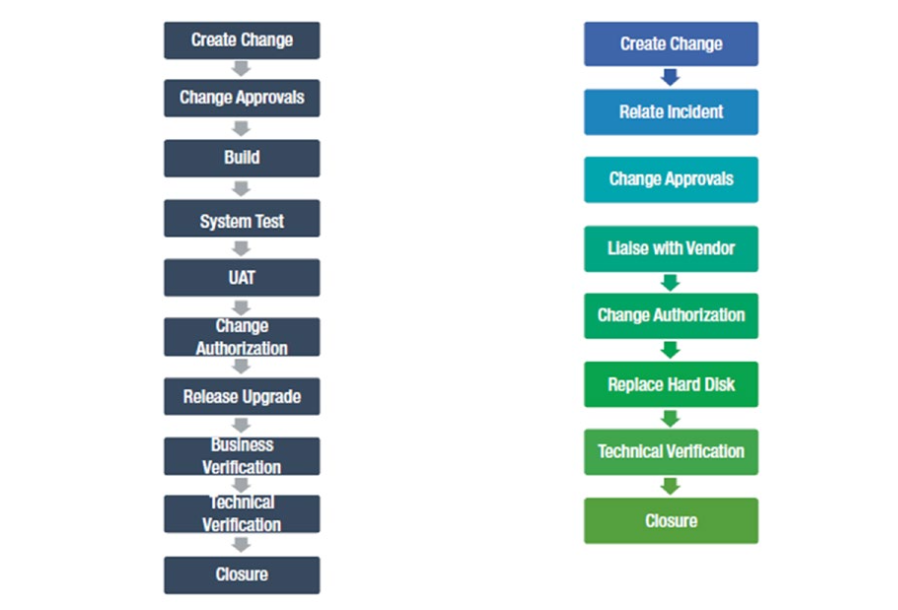
\includegraphics[width=0.5\linewidth]{images/image-02.png}
\end{center}
\end{frame}

\begin{frame}
	\frametitle{Normal Changes (cont.)}
	\begin{itemize}
		\item Different processes based on technology and policies
		\item Creation of change models for different types of changes
		\item Example: Software upgrade vs. hard disk replacement
		\item Change models define specific agreed-upon steps
		\item Improves delivery and governance of changes
	\end{itemize}
\end{frame}

\begin{frame}
	\frametitle{Emergency Changes}
	\begin{itemize}
		\item Urgently fix ongoing issues or crises
		\item Swift action with minimal planning
		\item Generally associated with major incidents
		\item Example: Replacing hardware infrastructure
		\item Support for incident management practice
		\item Reflects agility of the organization
	\end{itemize}
\end{frame}

\begin{frame}
	\frametitle{Standard Changes}
	\begin{itemize}
		\item Low risk and low impact
		\item Well understood and preapproved
		\item Examples: Minor patch upgrades, database reindexing
		\item Follow less stringent processes
		\item Increases productivity and value for customers
	\end{itemize}
\end{frame}

\begin{frame}
	\frametitle{Championing Standard Changes}
	\begin{itemize}
		\item Low-hanging value creation for clients
		\item Examples: Standard change processes, monitoring, and auditing
		\item Converts most routine changes into standard changes
		\item Benefits include cost savings and increased agility
	\end{itemize}
\end{frame}

\begin{frame}
	\frametitle{Change Advisory}
	\begin{itemize}
		\item Change authority advises change control practice
		\item Authorizes or rejects changes based on merit
		\item Decentralized change approvals for quick turnaround
		\item Local change authorities for different areas
		\item Primary change control body still central
	\end{itemize}
\end{frame}

\begin{frame}
	\frametitle{Change Schedule}
	\begin{itemize}
		\item Refers to a change calendar
		\item Includes changes in the pipeline and approved changes
		\item Helps in planning and avoiding conflicts
	\end{itemize}
\end{frame}

\begin{frame}{Multiple Choice Question}
	\textbf{Which of the following is the correct change definition?}
	
	\begin{enumerate}[A.]
		\item Any change of state that is significant for a service or product or related configuration item
		\item The addition, modification, or removal of anything that could have a direct or indirect effect on services
		\item Any change of state for configuration items that correlates risks and issues to the service and service management processes
		\item Any change that has significance for the management of a service or other additions, removals, and modifications
	\end{enumerate}
	
\end{frame}


\end{document}
